\chapter{Impact of Human specific variants on modern human biology}
\section{Introduction}
Uncovering genetic changes that make anatomically modern humans “unique” is critical for a comprehensive understanding of human evolution. Recent genomic advantages have began to elucidate the nuances of human evolution and how humankind relates to some of our closest hominid relatives. These advances are starting to reveal how intermixing between species has shaped modern human biology. Research has been done examining how regions of DNA that have been passed into homosapiens from our closest relatives, suggesting that some of this introgressed DNA may be adaptively beneficial or undergoing negative selection. On the other hand, there have been studies showing variant regions of DNA that are human-specific, or lacking in our closest relatives, suggesting that these mutations may have been important in developing modern human biology. 
%Some studies show (**add examples, foxp2,etc). 
One study used massively parallel reporter assays to look at regulatory effects of modern human specific variants \cite{weiss2021cis} in embryonic stem cells, neural progenitor cells, and bone osteoblasts finding (13\%) of sequences containing these variants showed active regulatory activity, and (23\%) of these drove differential expression between human groups. However, there hasn't been a comprehensive analysis determining and analysing the effect these mutations have on a broad range of human traits.
By analyzing genome sequences from our closest evolutionary relatives, Neanderthals and Denisovans, we can functionally characterize these genetic changes. Towards this end, we identified 50,505 mutations that are nearly fixed for the derived allele in African individuals from the 1000 Genomes project ($>90\%$ derived allele frequency) but are absent in all of the deeply sequenced Altai and Vindija Neanderthal and Denisovan genomes. Here we look at some of these human specific regions and how they impact modern human phenotypes.

To understand the phenotypic impact of these fixed derived mutations (FDMs), we leverage the observation that interbreeding with Neanderthals likely re-introduced the ancestral allele at a number of these sites. We estimate that $~39\%$ of FDMs are polymorphic in European populations so that their phenotypic impact can be analyzed by genotyping these mutations in large cohorts with phenotypic information.These Fixed Derived alleles (FDs) are mutations that rise to high frequency  in  modern  humans  since  the  split  from  archaic humans, and may give us clues to the biology that cause modern humans to differ from our closest relatives.
\section{Results}
\subsection{Identifying genomic regions at which fixed derived mutations influence phenotypes}
To understand how human specific mutations influence trait variation we first annotated the fixed derived mutations in the UK biobank. One approach we can use is to look at genetic components of traits that modern humans share, and our archaic relatives, such as the Neanderthal, don’t. In other words, we wanted to identify derived mutations in the modern human genome that differed from our ancient relatives, and rose to high frequency. These mutations occur after modern humans split from Archaic individuals such as Neanderthals, and then rise to a high frequency in modern humans. In order to overcome the problem of these mutations becoming fixed, or at nearly 100 \% allele frequency, we leverage the fact that introgression may have reintroduced variation into these mutations in European individuals (Fig 1). We first identified  25,448 (50,505) mutations that were $>99\% (>95\%)$ for the derived allele in 1000 genomes phase 3 African populations and ancestral in the Altai Neanderthal or Denisovan and deemed Fixed Derived mutations. These mutations are heterozygous in a number of White British individuals in the UK Biobank (Fig 2 \& 3). After identifying the $FDMs >99\%$, we used plink2 to run GLM on 96 phenotypes to find 464 FDMs associated with 39 phenotypes at a p-value threshold of $p<10^{-10}$.  For each phenotype, we clumped all significant FDMs that lie within 250 kb and with an LD threshold ($r^2$) of 0.5 using a significance threshold for the index SNP of $10^{-10}$. After clumping analysis we find 70 independent associations of the 39 phenotypes.

We repeated clumping analysis on $FDMs > 95\%$ and found 1457 FDM-phenotype associations over 67 phenotypes. 

We then performed our finemapping protocol as referenced in the previous section. 
\subsection{The contribution of FDMs to trait heritability}
%%%****FIX THIS LATER
To understand the contribution of human specific  variants to trait variation, we aim to estimate the proportion of phenotypic variance attributed to FDMs (FDMs heritability) and to test the null hypothesis that per-FDM heritability is the same as the heritability of a non-human specific SNP (MH) SNP. 
To estimate FDM heritability, we used a recently proposed method (RHE-mc) that can partition the heritability of a phenotype measured in large samples across various genomic annotations (Pazokitoroudi 2020). We applied RHE-mc with genomic annotations that correspond to the ancestry of each SNP (FDM vs MH) to estimate FDM heritability ($h^2_{FDM}$) as seen in Table \ref{table:4.1}. We also attempted to estimate whether per-FDM heritability is the same as the per-SNP heritability of MH SNPs ($\Delta_{h^2}$). A positive (negative) value of $\Delta_{h^2}$ indicates that, on average, a FDM makes a larger (smaller) contribution to phenotypic variation relative to a MH SNP. We found a number a traits in which FDMs made a smaller contribution to heritability than their counterparts. (Figs. \ref{fig:4.2} \ref{fig:4.3} \ref{fig:4.4}).
\section{Methods}
\subsection{UK Biobank (UKBB) genotype QC}
We restricted all our analyses to a set of high-quality imputed SNPs (with a hard call threshold of 0.2 and an info score greater than or equal to 0.8), which, among the 291,273 imputed genotypes of UKBB unrelated white British individuals, 1) have MAF higher than 0.001, 2) are under Hardy-Weinberg equilibrium ($p > 10^{-7}$), and 3) are confidently imputed in more than 99\% of the genomes. Additionally, we excluded SNPs in the MHC region, resulting in a total of 7,774,235 SNP which we refer to as QC-ed SNPs.
\subsection{Identifying Fixed Derived Mutations}
 We first determined derived allele frequencies from 504 African individuals in the 1000 genomes project phase3. We combined allele frequencies from ESN, GWD, LWK, MSL, YRI individuals in 1000 genomes in order to determine an African derived allele frequency for. We then determine the allele frequency in archaic individuals combining Vindija, and Altai neanderthals as well as the Denisovan individual. Combining the datasets, we examined 41,864,101 SNPs. We then filtered out SNPs with an African derived allele frequency >0.95 and >0.99 to find 50,505 and 25,448 mutations that are likely human specific. We then intersected these variants with those QC-ed SNPs in the UK Biobank to find 19,632 and 9,407 fixed derived mutations able to be tested.
 
\subsection{Association Testing}
To identify individual FDMs associated with a phenotype, we fit a linear regression model using plink 2.0 --glm and included covariates controlling for age, sex and the first 20 genotypic PCs, and first five FDM PCs. We used a stringent p-value threshold of $10^{-10}$ to correct for the number of FDMs and phenotypes tested. For each phenotype, we clumped all significant FDMs that lie within 250 kb and with an LD threshold ($r^2$) of 0.5 using a significance threshold for the index SNP of $10^{-10}$.


\subsection{Estimating FDM heritability with RHE-mc}
We are interested in estimating the proportion of phenotypic variance attributed to FDMss (true FDM heritability $h^2_{FDM}$) and evaluating if the heritability at a FDM (per-FDM heritability) is larger or smaller than that of a background MH SNP. To this end, we used a variance components model that partitions phenotypic variance across genomic annotations that include ancestry (FDM vs MH) as one of the input annotations.

We use RHE-mc, a method that can partition genetic variance across large sample sizes, to estimate FDM heritability (Pazokitoroudi 2020). For each phenotype, we run RHE-mc, in turn, with four types of input annotations: ancestry alone, ancestry + MAF, ancestry + LD, and ancestry + MAF + LD as described above. The ancestry+ MAF, ancestry + LD, and ancestry + MAF + LD annotations are intended to account for the differences in the MAF and LD properties of FDMs compared to MH SNPs.

To estimate FDM heritability, $\hat{h^2_{FDM}}$ , we combine the heritability of each bin corresponding to Neanderthal ancestry:

$$\hat{h^2_{FDM}} = \sum_i \hat{h^2_{FDM,i}}$$
and the heritability estimates for any bins with modern human ancestry are used to compute the total heritability from MH. Thus, when we estimate FDM heritability from RHE-mc run with ancestry + MAF annotations, we add the heritability estimates from five bins of low to high MAF FDMs.
 
To compare the average heritability at a FDM to the heritability of a background MH SNP that is chosen to match the FDM in terms of MAF and LD profiles, we compute the following statistic:
$$\hat{\Delta_{h^2}}=\hat{h^2_{FDM}}-\hat{h^2_{MH}}$$
where $\hat{h^2_{MH}} = \sum_i \frac{M_{FDM,i}}{M_{MH,i}} \hat{h^2_{MH,i}}$, iis the heritability of the background set matched for the MAF and LD profile of the set of FDMs. Here $M_{MH,i}$ denotes the number of MH SNPs in bin $i$  (defined according to MAF and/or LD of the MH SNPs) while $M_{FDM,i}$ denotes the number of FDMs in the corresponding bin. A more detailed justification of this statistic is provided in Note S4.

The standard errors (s.e.) of these statistics are computed using 100 jackknife blocks using an extension of RHE-mc that takes into account the covariance among different annotations. This new version of the RHE-mc is now available at https://github.com/alipazokit/RHEmc-coeff.
\newpage
\FloatBarrier
\section{Figures}
\begin{figure}[htb]
    \centering
    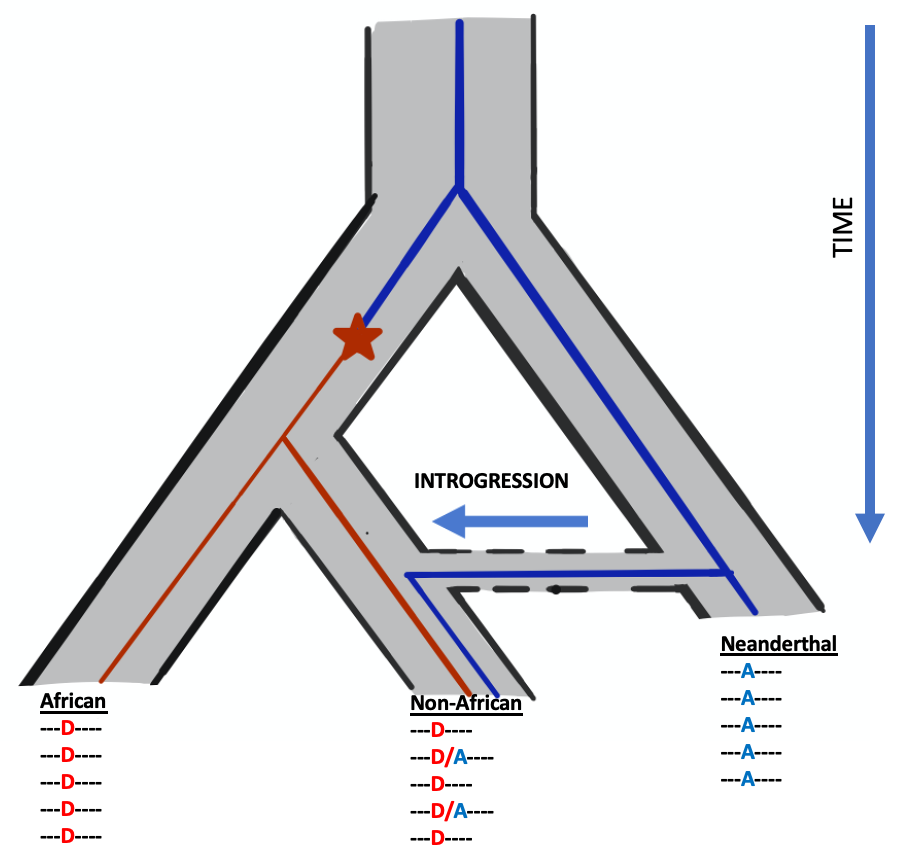
\includegraphics[width=\textwidth]{chapter4/figures/fig4.1.png}
    \caption{Cartoon depicting how Fixed Derived Mutations are determined}
    \label{fig:4.1}
\end{figure}

\begin{figure}[htb]
    \centering
    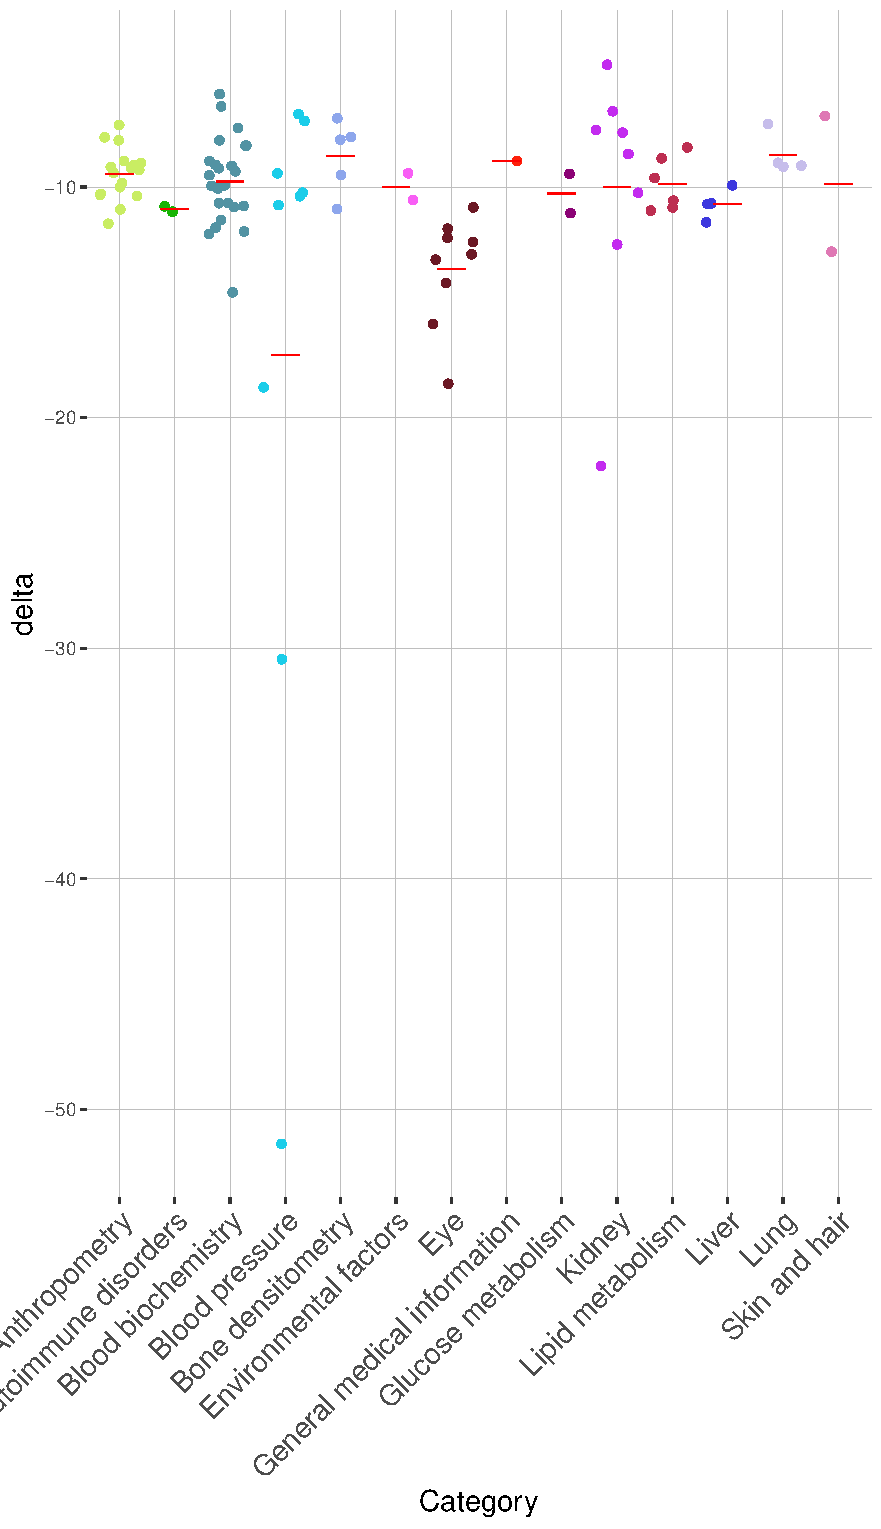
\includegraphics[width=\textwidth]{chapter4/figures/deltaplot.pdf}
    \caption{Enrichment of FDM heritability in each phenotype and category}
    \label{fig:4.2}
\end{figure}
\begin{figure}[htb]
    \centering
    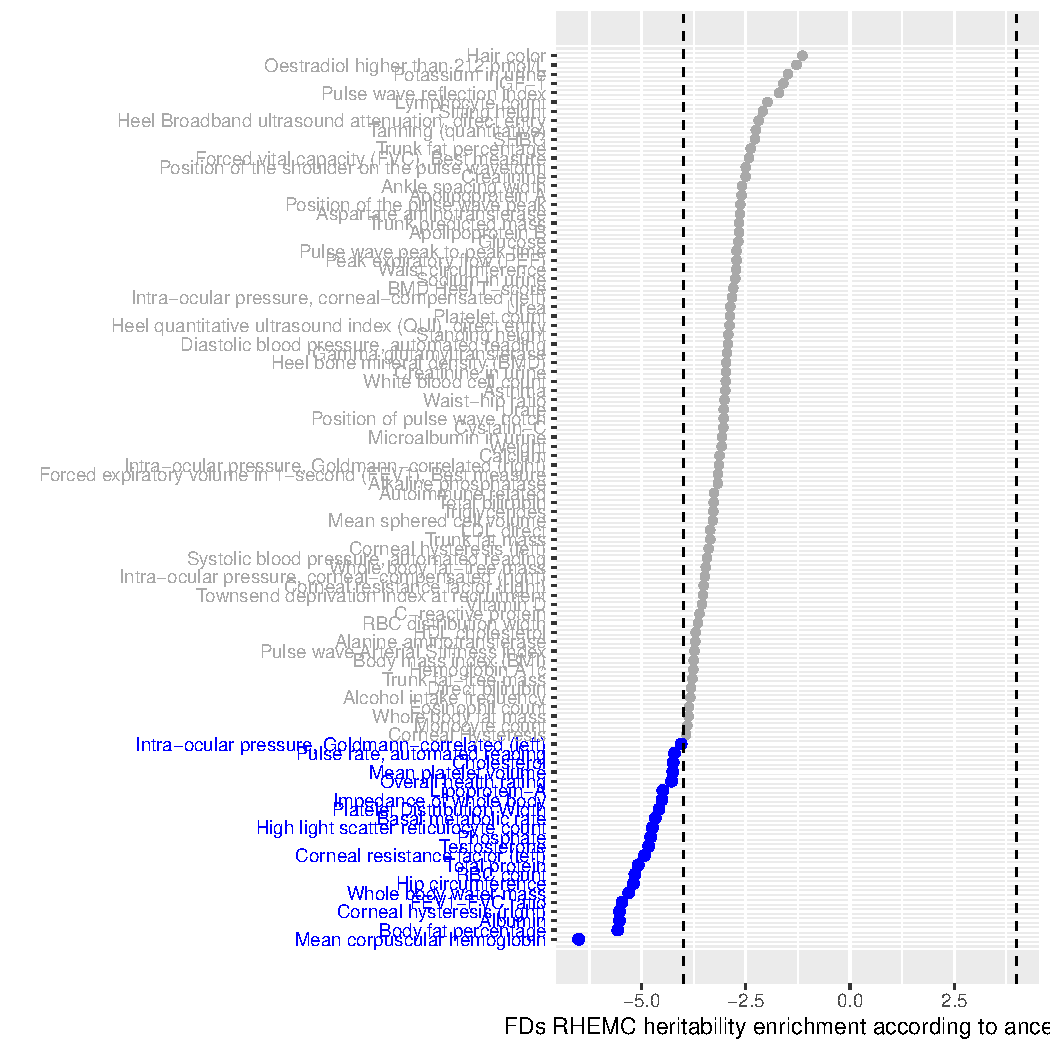
\includegraphics[]{chapter4/figures/fds.rhemc.z_nim_mh.pdf}
    \caption{FDs RHEMC heritability enrichment according to ancestry}
    \label{fig:4.3}
\end{figure}
\begin{figure}[htb]
    \centering
    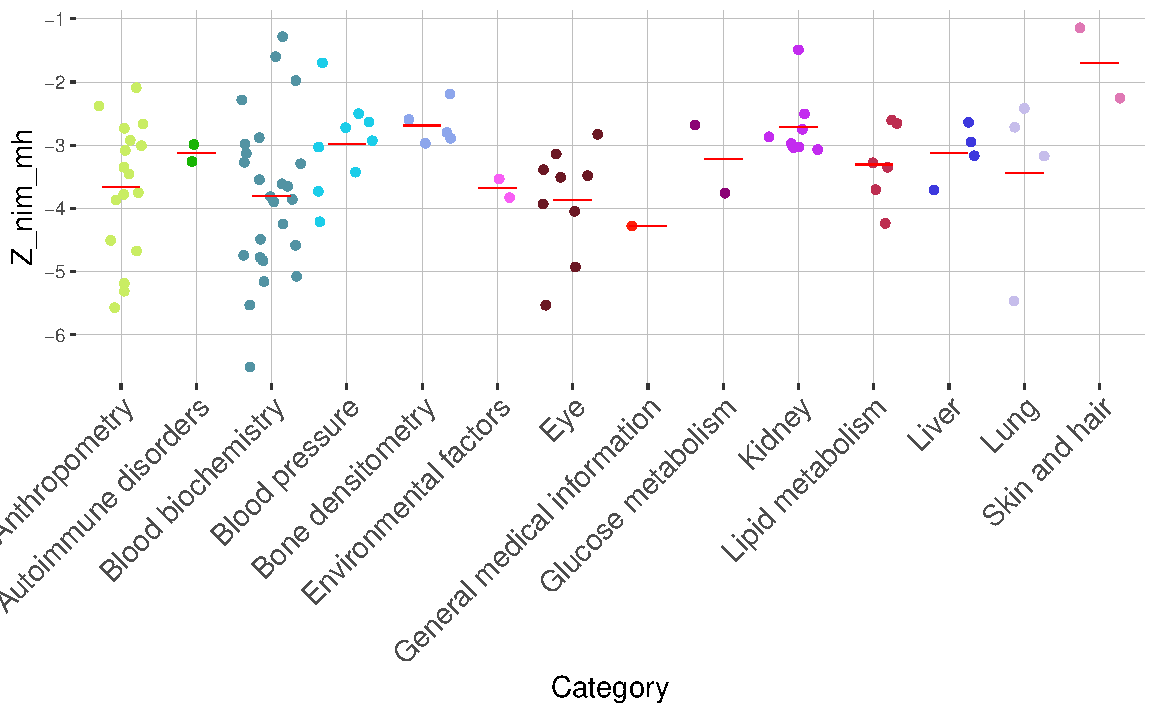
\includegraphics[width=\textwidth]{chapter4/figures/Z_nim_mh_category.pdf}
    \caption{Difference in heritability of FDMs vs modern humans by phenotype and category}
    \label{fig:4.4}
\end{figure}
\FloatBarrier
\section{Tables}
% Please add the following required packages to your document preamble:
% \usepackage{longtable}
% Note: It may be necessary to compile the document several times to get a multi-page table to line up properly
\begin{longtable}{llllllllllllll}
\hline
\textbf{fCode} &
  \textbf{Pheno} &
  \textbf{h2} &
  \textbf{h2(se)} &
  \textbf{z\_h2} &
  \textbf{h2\_FDM} &
  \textbf{h2\_FDM(se)} &
  \textbf{z\_FDM} &
  \textbf{h2\_mh} &
  \textbf{h2\_mh(se)} &
  \textbf{z\_mh} &
  \textbf{delta} &
  \textbf{delta(se)} &
  \textbf{Z\_FDM\_mh} \\ \hline
\endfirsthead
%
\multicolumn{14}{c}%
{{\bfseries Table \thetable\ continued from previous page}} \\
\endhead
%
\multicolumn{1}{|l|}{f.30620.0.0} &
  \multicolumn{1}{l|}{Alanine\_aminotransferase} &
  \multicolumn{1}{l|}{0.1445} &
  \multicolumn{1}{l|}{0.0143} &
  \multicolumn{1}{l|}{10.14} &
  \multicolumn{1}{l|}{-0.0020} &
  \multicolumn{1}{l|}{0.0005} &
  \multicolumn{1}{l|}{-4.13} &
  \multicolumn{1}{l|}{0.1465} &
  \multicolumn{1}{l|}{0.0141} &
  \multicolumn{1}{l|}{10.36} &
  \multicolumn{1}{l|}{-11.5266} &
  \multicolumn{1}{l|}{3.1053} &
  \multicolumn{1}{l|}{-3.71} \\ \hline
\multicolumn{1}{|l|}{f.30600.0.0} &
  \multicolumn{1}{l|}{Albumin} &
  \multicolumn{1}{l|}{0.1542} &
  \multicolumn{1}{l|}{0.0108} &
  \multicolumn{1}{l|}{14.29} &
  \multicolumn{1}{l|}{-0.0015} &
  \multicolumn{1}{l|}{0.0003} &
  \multicolumn{1}{l|}{-5.03} &
  \multicolumn{1}{l|}{0.1556} &
  \multicolumn{1}{l|}{0.0109} &
  \multicolumn{1}{l|}{14.28} &
  \multicolumn{1}{l|}{-7.9751} &
  \multicolumn{1}{l|}{1.4426} &
  \multicolumn{1}{l|}{-5.53} \\ \hline
\multicolumn{1}{|l|}{f.1558.0.0} &
  \multicolumn{1}{l|}{Alcohol\_intake\_frequency} &
  \multicolumn{1}{l|}{0.1054} &
  \multicolumn{1}{l|}{0.0071} &
  \multicolumn{1}{l|}{14.88} &
  \multicolumn{1}{l|}{-0.0012} &
  \multicolumn{1}{l|}{0.0003} &
  \multicolumn{1}{l|}{-4.33} &
  \multicolumn{1}{l|}{0.1066} &
  \multicolumn{1}{l|}{0.0070} &
  \multicolumn{1}{l|}{15.33} &
  \multicolumn{1}{l|}{-9.4013} &
  \multicolumn{1}{l|}{2.4529} &
  \multicolumn{1}{l|}{-3.83} \\ \hline
\multicolumn{1}{|l|}{f.30610.0.0} &
  \multicolumn{1}{l|}{Alkaline\_phosphatase} &
  \multicolumn{1}{l|}{0.3059} &
  \multicolumn{1}{l|}{0.0573} &
  \multicolumn{1}{l|}{5.33} &
  \multicolumn{1}{l|}{-0.0037} &
  \multicolumn{1}{l|}{0.0012} &
  \multicolumn{1}{l|}{-2.98} &
  \multicolumn{1}{l|}{0.3096} &
  \multicolumn{1}{l|}{0.0577} &
  \multicolumn{1}{l|}{5.36} &
  \multicolumn{1}{l|}{-9.9234} &
  \multicolumn{1}{l|}{3.1314} &
  \multicolumn{1}{l|}{-3.17} \\ \hline
\multicolumn{1}{|l|}{f.30630.0.0} &
  \multicolumn{1}{l|}{Apolipoprotein\_A} &
  \multicolumn{1}{l|}{0.2444} &
  \multicolumn{1}{l|}{0.0317} &
  \multicolumn{1}{l|}{7.70} &
  \multicolumn{1}{l|}{-0.0033} &
  \multicolumn{1}{l|}{0.0012} &
  \multicolumn{1}{l|}{-2.66} &
  \multicolumn{1}{l|}{0.2476} &
  \multicolumn{1}{l|}{0.0318} &
  \multicolumn{1}{l|}{7.79} &
  \multicolumn{1}{l|}{-11.0198} &
  \multicolumn{1}{l|}{4.2345} &
  \multicolumn{1}{l|}{-2.60} \\ \hline
\multicolumn{1}{|l|}{f.30640.0.0} &
  \multicolumn{1}{l|}{Apolipoprotein\_B} &
  \multicolumn{1}{l|}{0.1451} &
  \multicolumn{1}{l|}{0.0317} &
  \multicolumn{1}{l|}{4.58} &
  \multicolumn{1}{l|}{-0.0019} &
  \multicolumn{1}{l|}{0.0008} &
  \multicolumn{1}{l|}{-2.50} &
  \multicolumn{1}{l|}{0.1470} &
  \multicolumn{1}{l|}{0.0319} &
  \multicolumn{1}{l|}{4.61} &
  \multicolumn{1}{l|}{-10.8829} &
  \multicolumn{1}{l|}{4.0918} &
  \multicolumn{1}{l|}{-2.66} \\ \hline
\multicolumn{1}{|l|}{f.30650.0.0} &
  \multicolumn{1}{l|}{Aspartate\_aminotransferase} &
  \multicolumn{1}{l|}{0.1582} &
  \multicolumn{1}{l|}{0.0165} &
  \multicolumn{1}{l|}{9.60} &
  \multicolumn{1}{l|}{-0.0021} &
  \multicolumn{1}{l|}{0.0007} &
  \multicolumn{1}{l|}{-2.86} &
  \multicolumn{1}{l|}{0.1602} &
  \multicolumn{1}{l|}{0.0163} &
  \multicolumn{1}{l|}{9.86} &
  \multicolumn{1}{l|}{-10.7322} &
  \multicolumn{1}{l|}{4.0697} &
  \multicolumn{1}{l|}{-2.64} \\ \hline
\multicolumn{1}{|l|}{f.6152.0.0} &
  \multicolumn{1}{l|}{Asthma} &
  \multicolumn{1}{l|}{0.0999} &
  \multicolumn{1}{l|}{0.0098} &
  \multicolumn{1}{l|}{10.19} &
  \multicolumn{1}{l|}{-0.0013} &
  \multicolumn{1}{l|}{0.0004} &
  \multicolumn{1}{l|}{-3.27} &
  \multicolumn{1}{l|}{0.1012} &
  \multicolumn{1}{l|}{0.0097} &
  \multicolumn{1}{l|}{10.45} &
  \multicolumn{1}{l|}{-10.8349} &
  \multicolumn{1}{l|}{3.6236} &
  \multicolumn{1}{l|}{-2.99} \\ \hline
\multicolumn{1}{|l|}{f.20002} &
  \multicolumn{1}{l|}{Autoimmune\_related} &
  \multicolumn{1}{l|}{0.0541} &
  \multicolumn{1}{l|}{0.0055} &
  \multicolumn{1}{l|}{9.85} &
  \multicolumn{1}{l|}{-0.0007} &
  \multicolumn{1}{l|}{0.0002} &
  \multicolumn{1}{l|}{-3.47} &
  \multicolumn{1}{l|}{0.0548} &
  \multicolumn{1}{l|}{0.0055} &
  \multicolumn{1}{l|}{10.03} &
  \multicolumn{1}{l|}{-11.0694} &
  \multicolumn{1}{l|}{3.3979} &
  \multicolumn{1}{l|}{-3.26} \\ \hline
\multicolumn{1}{|l|}{f.23105.0.0} &
  \multicolumn{1}{l|}{Basal\_metabolic\_rate} &
  \multicolumn{1}{l|}{0.3474} &
  \multicolumn{1}{l|}{0.0211} &
  \multicolumn{1}{l|}{16.50} &
  \multicolumn{1}{l|}{-0.0038} &
  \multicolumn{1}{l|}{0.0008} &
  \multicolumn{1}{l|}{-5.05} &
  \multicolumn{1}{l|}{0.3512} &
  \multicolumn{1}{l|}{0.0209} &
  \multicolumn{1}{l|}{16.81} &
  \multicolumn{1}{l|}{-9.1212} &
  \multicolumn{1}{l|}{1.9547} &
  \multicolumn{1}{l|}{-4.67} \\ \hline
\multicolumn{1}{|l|}{f.30660.0.0} &
  \multicolumn{1}{l|}{Direct\_bilirubin} &
  \multicolumn{1}{l|}{0.3399} &
  \multicolumn{1}{l|}{0.2642} &
  \multicolumn{1}{l|}{1.29} &
  \multicolumn{1}{l|}{-0.0048} &
  \multicolumn{1}{l|}{0.0039} &
  \multicolumn{1}{l|}{-1.23} &
  \multicolumn{1}{l|}{0.3447} &
  \multicolumn{1}{l|}{0.2679} &
  \multicolumn{1}{l|}{1.29} &
  \multicolumn{1}{l|}{-11.7598} &
  \multicolumn{1}{l|}{3.0828} &
  \multicolumn{1}{l|}{-3.81} \\ \hline
\multicolumn{1}{|l|}{f.30840.0.0} &
  \multicolumn{1}{l|}{Total\_bilirubin} &
  \multicolumn{1}{l|}{0.4560} &
  \multicolumn{1}{l|}{0.3465} &
  \multicolumn{1}{l|}{1.32} &
  \multicolumn{1}{l|}{-0.0066} &
  \multicolumn{1}{l|}{0.0055} &
  \multicolumn{1}{l|}{-1.21} &
  \multicolumn{1}{l|}{0.4627} &
  \multicolumn{1}{l|}{0.3517} &
  \multicolumn{1}{l|}{1.32} &
  \multicolumn{1}{l|}{-12.0399} &
  \multicolumn{1}{l|}{3.6865} &
  \multicolumn{1}{l|}{-3.27} \\ \hline
\multicolumn{1}{|l|}{f.30150.0.0} &
  \multicolumn{1}{l|}{Eosinophil\_count} &
  \multicolumn{1}{l|}{0.2466} &
  \multicolumn{1}{l|}{0.0253} &
  \multicolumn{1}{l|}{9.76} &
  \multicolumn{1}{l|}{-0.0030} &
  \multicolumn{1}{l|}{0.0008} &
  \multicolumn{1}{l|}{-3.92} &
  \multicolumn{1}{l|}{0.2496} &
  \multicolumn{1}{l|}{0.0253} &
  \multicolumn{1}{l|}{9.85} &
  \multicolumn{1}{l|}{-10.0594} &
  \multicolumn{1}{l|}{2.6064} &
  \multicolumn{1}{l|}{-3.86} \\ \hline
\multicolumn{1}{|l|}{f.30120.0.0} &
  \multicolumn{1}{l|}{Lymphocyte\_count} &
  \multicolumn{1}{l|}{0.2291} &
  \multicolumn{1}{l|}{0.0262} &
  \multicolumn{1}{l|}{8.74} &
  \multicolumn{1}{l|}{-0.0033} &
  \multicolumn{1}{l|}{0.0015} &
  \multicolumn{1}{l|}{-2.18} &
  \multicolumn{1}{l|}{0.2324} &
  \multicolumn{1}{l|}{0.0253} &
  \multicolumn{1}{l|}{9.20} &
  \multicolumn{1}{l|}{-11.9284} &
  \multicolumn{1}{l|}{6.0357} &
  \multicolumn{1}{l|}{-1.98} \\ \hline
\multicolumn{1}{|l|}{f.30050.0.0} &
  \multicolumn{1}{l|}{Mean\_corpuscular\_hemoglobin} &
  \multicolumn{1}{l|}{0.2874} &
  \multicolumn{1}{l|}{0.0292} &
  \multicolumn{1}{l|}{9.86} &
  \multicolumn{1}{l|}{-0.0032} &
  \multicolumn{1}{l|}{0.0006} &
  \multicolumn{1}{l|}{-5.27} &
  \multicolumn{1}{l|}{0.2907} &
  \multicolumn{1}{l|}{0.0295} &
  \multicolumn{1}{l|}{9.85} &
  \multicolumn{1}{l|}{-9.3155} &
  \multicolumn{1}{l|}{1.4316} &
  \multicolumn{1}{l|}{-6.51} \\ \hline
\multicolumn{1}{|l|}{f.30130.0.0} &
  \multicolumn{1}{l|}{Monocyte\_count} &
  \multicolumn{1}{l|}{0.2484} &
  \multicolumn{1}{l|}{0.0278} &
  \multicolumn{1}{l|}{8.95} &
  \multicolumn{1}{l|}{-0.0020} &
  \multicolumn{1}{l|}{0.0005} &
  \multicolumn{1}{l|}{-3.84} &
  \multicolumn{1}{l|}{0.2503} &
  \multicolumn{1}{l|}{0.0279} &
  \multicolumn{1}{l|}{8.97} &
  \multicolumn{1}{l|}{-6.4998} &
  \multicolumn{1}{l|}{1.6678} &
  \multicolumn{1}{l|}{-3.90} \\ \hline
\multicolumn{1}{|l|}{f.30100.0.0} &
  \multicolumn{1}{l|}{Mean\_platelet\_volume} &
  \multicolumn{1}{l|}{0.4147} &
  \multicolumn{1}{l|}{0.0503} &
  \multicolumn{1}{l|}{8.25} &
  \multicolumn{1}{l|}{-0.0045} &
  \multicolumn{1}{l|}{0.0011} &
  \multicolumn{1}{l|}{-4.13} &
  \multicolumn{1}{l|}{0.4192} &
  \multicolumn{1}{l|}{0.0506} &
  \multicolumn{1}{l|}{8.29} &
  \multicolumn{1}{l|}{-8.8739} &
  \multicolumn{1}{l|}{2.0902} &
  \multicolumn{1}{l|}{-4.25} \\ \hline
\multicolumn{1}{|l|}{f.30270.0.0} &
  \multicolumn{1}{l|}{Mean\_sphered\_cell\_volume} &
  \multicolumn{1}{l|}{0.2379} &
  \multicolumn{1}{l|}{0.0285} &
  \multicolumn{1}{l|}{8.36} &
  \multicolumn{1}{l|}{-0.0031} &
  \multicolumn{1}{l|}{0.0008} &
  \multicolumn{1}{l|}{-3.63} &
  \multicolumn{1}{l|}{0.2410} &
  \multicolumn{1}{l|}{0.0283} &
  \multicolumn{1}{l|}{8.51} &
  \multicolumn{1}{l|}{-10.6986} &
  \multicolumn{1}{l|}{3.2521} &
  \multicolumn{1}{l|}{-3.29} \\ \hline
\multicolumn{1}{|l|}{f.30110.0.0} &
  \multicolumn{1}{l|}{Platelet\_Distribution\_Width} &
  \multicolumn{1}{l|}{0.2902} &
  \multicolumn{1}{l|}{0.0343} &
  \multicolumn{1}{l|}{8.45} &
  \multicolumn{1}{l|}{-0.0032} &
  \multicolumn{1}{l|}{0.0007} &
  \multicolumn{1}{l|}{-4.39} &
  \multicolumn{1}{l|}{0.2934} &
  \multicolumn{1}{l|}{0.0346} &
  \multicolumn{1}{l|}{8.49} &
  \multicolumn{1}{l|}{-9.0367} &
  \multicolumn{1}{l|}{1.9725} &
  \multicolumn{1}{l|}{-4.58} \\ \hline
\multicolumn{1}{|l|}{f.30080.0.0} &
  \multicolumn{1}{l|}{Platelet\_count} &
  \multicolumn{1}{l|}{0.3012} &
  \multicolumn{1}{l|}{0.0342} &
  \multicolumn{1}{l|}{8.81} &
  \multicolumn{1}{l|}{-0.0040} &
  \multicolumn{1}{l|}{0.0012} &
  \multicolumn{1}{l|}{-3.32} &
  \multicolumn{1}{l|}{0.3051} &
  \multicolumn{1}{l|}{0.0336} &
  \multicolumn{1}{l|}{9.07} &
  \multicolumn{1}{l|}{-10.8684} &
  \multicolumn{1}{l|}{3.7748} &
  \multicolumn{1}{l|}{-2.88} \\ \hline
\multicolumn{1}{|l|}{f.30010.0.0} &
  \multicolumn{1}{l|}{RBC\_count} &
  \multicolumn{1}{l|}{0.2629} &
  \multicolumn{1}{l|}{0.0224} &
  \multicolumn{1}{l|}{11.75} &
  \multicolumn{1}{l|}{-0.0032} &
  \multicolumn{1}{l|}{0.0006} &
  \multicolumn{1}{l|}{-5.34} &
  \multicolumn{1}{l|}{0.2661} &
  \multicolumn{1}{l|}{0.0224} &
  \multicolumn{1}{l|}{11.87} &
  \multicolumn{1}{l|}{-9.9243} &
  \multicolumn{1}{l|}{1.9223} &
  \multicolumn{1}{l|}{-5.16} \\ \hline
\multicolumn{1}{|l|}{f.30030.0.0} &
  \multicolumn{1}{l|}{RBC\_distribution\_width} &
  \multicolumn{1}{l|}{0.2355} &
  \multicolumn{1}{l|}{0.0246} &
  \multicolumn{1}{l|}{9.59} &
  \multicolumn{1}{l|}{-0.0028} &
  \multicolumn{1}{l|}{0.0007} &
  \multicolumn{1}{l|}{-3.83} &
  \multicolumn{1}{l|}{0.2383} &
  \multicolumn{1}{l|}{0.0246} &
  \multicolumn{1}{l|}{9.70} &
  \multicolumn{1}{l|}{-9.9634} &
  \multicolumn{1}{l|}{2.7327} &
  \multicolumn{1}{l|}{-3.65} \\ \hline
\multicolumn{1}{|l|}{f.30300.0.0} &
  \multicolumn{1}{l|}{High\_light\_scatter\_reticulocyte\_count} &
  \multicolumn{1}{l|}{0.2836} &
  \multicolumn{1}{l|}{0.0286} &
  \multicolumn{1}{l|}{9.92} &
  \multicolumn{1}{l|}{-0.0032} &
  \multicolumn{1}{l|}{0.0007} &
  \multicolumn{1}{l|}{-4.56} &
  \multicolumn{1}{l|}{0.2868} &
  \multicolumn{1}{l|}{0.0288} &
  \multicolumn{1}{l|}{9.96} &
  \multicolumn{1}{l|}{-9.1811} &
  \multicolumn{1}{l|}{1.9373} &
  \multicolumn{1}{l|}{-4.74} \\ \hline
\multicolumn{1}{|l|}{f.30000.0.0} &
  \multicolumn{1}{l|}{White\_blood\_cell\_count} &
  \multicolumn{1}{l|}{0.2240} &
  \multicolumn{1}{l|}{0.0221} &
  \multicolumn{1}{l|}{10.13} &
  \multicolumn{1}{l|}{-0.0029} &
  \multicolumn{1}{l|}{0.0009} &
  \multicolumn{1}{l|}{-3.31} &
  \multicolumn{1}{l|}{0.2269} &
  \multicolumn{1}{l|}{0.0218} &
  \multicolumn{1}{l|}{10.40} &
  \multicolumn{1}{l|}{-10.6907} &
  \multicolumn{1}{l|}{3.5816} &
  \multicolumn{1}{l|}{-2.98} \\ \hline
\multicolumn{1}{|l|}{f.4106.0.0+f.4125.0.0} &
  \multicolumn{1}{l|}{BMD\_Heel\_T-score} &
  \multicolumn{1}{l|}{0.3690} &
  \multicolumn{1}{l|}{0.0344} &
  \multicolumn{1}{l|}{10.73} &
  \multicolumn{1}{l|}{-0.0049} &
  \multicolumn{1}{l|}{0.0017} &
  \multicolumn{1}{l|}{-2.89} &
  \multicolumn{1}{l|}{0.3739} &
  \multicolumn{1}{l|}{0.0343} &
  \multicolumn{1}{l|}{10.90} &
  \multicolumn{1}{l|}{-10.9474} &
  \multicolumn{1}{l|}{3.9124} &
  \multicolumn{1}{l|}{-2.80} \\ \hline
\multicolumn{1}{|l|}{f.30680.0.0} &
  \multicolumn{1}{l|}{Calcium} &
  \multicolumn{1}{l|}{0.1561} &
  \multicolumn{1}{l|}{0.0214} &
  \multicolumn{1}{l|}{7.29} &
  \multicolumn{1}{l|}{-0.0015} &
  \multicolumn{1}{l|}{0.0005} &
  \multicolumn{1}{l|}{-2.95} &
  \multicolumn{1}{l|}{0.1576} &
  \multicolumn{1}{l|}{0.0216} &
  \multicolumn{1}{l|}{7.30} &
  \multicolumn{1}{l|}{-8.2066} &
  \multicolumn{1}{l|}{2.6198} &
  \multicolumn{1}{l|}{-3.13} \\ \hline
\multicolumn{1}{|l|}{f.30690.0.0} &
  \multicolumn{1}{l|}{Cholesterol} &
  \multicolumn{1}{l|}{0.1417} &
  \multicolumn{1}{l|}{0.0189} &
  \multicolumn{1}{l|}{7.50} &
  \multicolumn{1}{l|}{-0.0014} &
  \multicolumn{1}{l|}{0.0004} &
  \multicolumn{1}{l|}{-3.74} &
  \multicolumn{1}{l|}{0.1432} &
  \multicolumn{1}{l|}{0.0191} &
  \multicolumn{1}{l|}{7.50} &
  \multicolumn{1}{l|}{-8.2814} &
  \multicolumn{1}{l|}{1.9513} &
  \multicolumn{1}{l|}{-4.24} \\ \hline
\multicolumn{1}{|l|}{f.5256.0.0+f.5264.0.0} &
  \multicolumn{1}{l|}{Corneal\_Hysteresis} &
  \multicolumn{1}{l|}{0.2900} &
  \multicolumn{1}{l|}{0.0265} &
  \multicolumn{1}{l|}{10.96} &
  \multicolumn{1}{l|}{-0.0046} &
  \multicolumn{1}{l|}{0.0010} &
  \multicolumn{1}{l|}{-4.49} &
  \multicolumn{1}{l|}{0.2946} &
  \multicolumn{1}{l|}{0.0262} &
  \multicolumn{1}{l|}{11.23} &
  \multicolumn{1}{l|}{-13.1479} &
  \multicolumn{1}{l|}{3.3443} &
  \multicolumn{1}{l|}{-3.93} \\ \hline
\multicolumn{1}{|l|}{f.30710.0.0} &
  \multicolumn{1}{l|}{C-reactive\_protein} &
  \multicolumn{1}{l|}{0.2379} &
  \multicolumn{1}{l|}{0.0352} &
  \multicolumn{1}{l|}{6.76} &
  \multicolumn{1}{l|}{-0.0026} &
  \multicolumn{1}{l|}{0.0008} &
  \multicolumn{1}{l|}{-3.24} &
  \multicolumn{1}{l|}{0.2405} &
  \multicolumn{1}{l|}{0.0355} &
  \multicolumn{1}{l|}{6.77} &
  \multicolumn{1}{l|}{-9.0857} &
  \multicolumn{1}{l|}{2.5163} &
  \multicolumn{1}{l|}{-3.61} \\ \hline
\multicolumn{1}{|l|}{f.30700.0.0} &
  \multicolumn{1}{l|}{Creatinine} &
  \multicolumn{1}{l|}{0.2433} &
  \multicolumn{1}{l|}{0.0163} &
  \multicolumn{1}{l|}{14.93} &
  \multicolumn{1}{l|}{-0.0020} &
  \multicolumn{1}{l|}{0.0008} &
  \multicolumn{1}{l|}{-2.56} &
  \multicolumn{1}{l|}{0.2453} &
  \multicolumn{1}{l|}{0.0162} &
  \multicolumn{1}{l|}{15.15} &
  \multicolumn{1}{l|}{-6.7094} &
  \multicolumn{1}{l|}{2.6882} &
  \multicolumn{1}{l|}{-2.50} \\ \hline
\multicolumn{1}{|l|}{f.30510.0.0} &
  \multicolumn{1}{l|}{Creatinine\_in\_urine} &
  \multicolumn{1}{l|}{0.0754} &
  \multicolumn{1}{l|}{0.0044} &
  \multicolumn{1}{l|}{17.01} &
  \multicolumn{1}{l|}{-0.0007} &
  \multicolumn{1}{l|}{0.0002} &
  \multicolumn{1}{l|}{-3.19} &
  \multicolumn{1}{l|}{0.0761} &
  \multicolumn{1}{l|}{0.0044} &
  \multicolumn{1}{l|}{17.48} &
  \multicolumn{1}{l|}{-7.6378} &
  \multicolumn{1}{l|}{2.5690} &
  \multicolumn{1}{l|}{-2.97} \\ \hline
\multicolumn{1}{|l|}{f.30720.0.0} &
  \multicolumn{1}{l|}{Cystatin-C} &
  \multicolumn{1}{l|}{0.3282} &
  \multicolumn{1}{l|}{0.1032} &
  \multicolumn{1}{l|}{3.18} &
  \multicolumn{1}{l|}{-0.0034} &
  \multicolumn{1}{l|}{0.0017} &
  \multicolumn{1}{l|}{-2.04} &
  \multicolumn{1}{l|}{0.3316} &
  \multicolumn{1}{l|}{0.1046} &
  \multicolumn{1}{l|}{3.17} &
  \multicolumn{1}{l|}{-8.5644} &
  \multicolumn{1}{l|}{2.8154} &
  \multicolumn{1}{l|}{-3.04} \\ \hline
\multicolumn{1}{|l|}{f.102.0.0} &
  \multicolumn{1}{l|}{Pulse\_rate,\_automated\_reading} &
  \multicolumn{1}{l|}{0.1717} &
  \multicolumn{1}{l|}{0.0164} &
  \multicolumn{1}{l|}{10.48} &
  \multicolumn{1}{l|}{-0.0020} &
  \multicolumn{1}{l|}{0.0004} &
  \multicolumn{1}{l|}{-4.51} &
  \multicolumn{1}{l|}{0.1737} &
  \multicolumn{1}{l|}{0.0164} &
  \multicolumn{1}{l|}{10.61} &
  \multicolumn{1}{l|}{-9.4053} &
  \multicolumn{1}{l|}{2.2339} &
  \multicolumn{1}{l|}{-4.21} \\ \hline
\multicolumn{1}{|l|}{f.189.0.0} &
  \multicolumn{1}{l|}{Townsend\_deprivation\_index\_at\_recruitment} &
  \multicolumn{1}{l|}{0.0477} &
  \multicolumn{1}{l|}{0.0038} &
  \multicolumn{1}{l|}{12.65} &
  \multicolumn{1}{l|}{-0.0006} &
  \multicolumn{1}{l|}{0.0002} &
  \multicolumn{1}{l|}{-3.88} &
  \multicolumn{1}{l|}{0.0483} &
  \multicolumn{1}{l|}{0.0037} &
  \multicolumn{1}{l|}{12.96} &
  \multicolumn{1}{l|}{-10.5596} &
  \multicolumn{1}{l|}{2.9886} &
  \multicolumn{1}{l|}{-3.53} \\ \hline
\multicolumn{1}{|l|}{f.20015.0.0} &
  \multicolumn{1}{l|}{Sitting\_height} &
  \multicolumn{1}{l|}{0.3932} &
  \multicolumn{1}{l|}{0.0452} &
  \multicolumn{1}{l|}{8.69} &
  \multicolumn{1}{l|}{-0.0052} &
  \multicolumn{1}{l|}{0.0022} &
  \multicolumn{1}{l|}{-2.33} &
  \multicolumn{1}{l|}{0.3984} &
  \multicolumn{1}{l|}{0.0439} &
  \multicolumn{1}{l|}{9.08} &
  \multicolumn{1}{l|}{-10.9696} &
  \multicolumn{1}{l|}{5.2372} &
  \multicolumn{1}{l|}{-2.09} \\ \hline
\multicolumn{1}{|l|}{f.20150.0.0} &
  \multicolumn{1}{l|}{Forced\_expiratory\_volume\_in\_1-second\_(FEV1),\_Best\_measure} &
  \multicolumn{1}{l|}{0.2597} &
  \multicolumn{1}{l|}{0.0168} &
  \multicolumn{1}{l|}{15.49} &
  \multicolumn{1}{l|}{-0.0023} &
  \multicolumn{1}{l|}{0.0007} &
  \multicolumn{1}{l|}{-3.33} &
  \multicolumn{1}{l|}{0.2619} &
  \multicolumn{1}{l|}{0.0167} &
  \multicolumn{1}{l|}{15.72} &
  \multicolumn{1}{l|}{-7.2605} &
  \multicolumn{1}{l|}{2.2874} &
  \multicolumn{1}{l|}{-3.17} \\ \hline
\multicolumn{1}{|l|}{f.20151.0.0} &
  \multicolumn{1}{l|}{Forced\_vital\_capacity\_(FVC),\_Best\_measure} &
  \multicolumn{1}{l|}{0.2892} &
  \multicolumn{1}{l|}{0.0214} &
  \multicolumn{1}{l|}{13.49} &
  \multicolumn{1}{l|}{-0.0032} &
  \multicolumn{1}{l|}{0.0012} &
  \multicolumn{1}{l|}{-2.61} &
  \multicolumn{1}{l|}{0.2924} &
  \multicolumn{1}{l|}{0.0209} &
  \multicolumn{1}{l|}{13.97} &
  \multicolumn{1}{l|}{-9.0695} &
  \multicolumn{1}{l|}{3.7403} &
  \multicolumn{1}{l|}{-2.42} \\ \hline
\multicolumn{1}{|l|}{f.21001.0.0} &
  \multicolumn{1}{l|}{Body\_mass\_index\_(BMI)} &
  \multicolumn{1}{l|}{0.2861} &
  \multicolumn{1}{l|}{0.0242} &
  \multicolumn{1}{l|}{11.80} &
  \multicolumn{1}{l|}{-0.0036} &
  \multicolumn{1}{l|}{0.0008} &
  \multicolumn{1}{l|}{-4.59} &
  \multicolumn{1}{l|}{0.2897} &
  \multicolumn{1}{l|}{0.0237} &
  \multicolumn{1}{l|}{12.20} &
  \multicolumn{1}{l|}{-10.3354} &
  \multicolumn{1}{l|}{2.7588} &
  \multicolumn{1}{l|}{-3.75} \\ \hline
\multicolumn{1}{|l|}{f.21002.0.0} &
  \multicolumn{1}{l|}{Weight} &
  \multicolumn{1}{l|}{0.2961} &
  \multicolumn{1}{l|}{0.0231} &
  \multicolumn{1}{l|}{12.84} &
  \multicolumn{1}{l|}{-0.0042} &
  \multicolumn{1}{l|}{0.0012} &
  \multicolumn{1}{l|}{-3.55} &
  \multicolumn{1}{l|}{0.3002} &
  \multicolumn{1}{l|}{0.0223} &
  \multicolumn{1}{l|}{13.48} &
  \multicolumn{1}{l|}{-11.5919} &
  \multicolumn{1}{l|}{3.7675} &
  \multicolumn{1}{l|}{-3.08} \\ \hline
\multicolumn{1}{|l|}{f.21021.0.0} &
  \multicolumn{1}{l|}{Pulse\_wave\_Arterial\_Stiffness\_index} &
  \multicolumn{1}{l|}{0.0329} &
  \multicolumn{1}{l|}{0.0066} &
  \multicolumn{1}{l|}{5.00} &
  \multicolumn{1}{l|}{-0.0012} &
  \multicolumn{1}{l|}{0.0003} &
  \multicolumn{1}{l|}{-4.65} &
  \multicolumn{1}{l|}{0.0341} &
  \multicolumn{1}{l|}{0.0066} &
  \multicolumn{1}{l|}{5.16} &
  \multicolumn{1}{l|}{-30.4793} &
  \multicolumn{1}{l|}{8.1812} &
  \multicolumn{1}{l|}{-3.73} \\ \hline
\multicolumn{1}{|l|}{f.23099.0.0} &
  \multicolumn{1}{l|}{Body\_fat\_percentage} &
  \multicolumn{1}{l|}{0.2929} &
  \multicolumn{1}{l|}{0.0140} &
  \multicolumn{1}{l|}{20.86} &
  \multicolumn{1}{l|}{-0.0026} &
  \multicolumn{1}{l|}{0.0004} &
  \multicolumn{1}{l|}{-5.83} &
  \multicolumn{1}{l|}{0.2955} &
  \multicolumn{1}{l|}{0.0140} &
  \multicolumn{1}{l|}{21.08} &
  \multicolumn{1}{l|}{-7.3107} &
  \multicolumn{1}{l|}{1.3115} &
  \multicolumn{1}{l|}{-5.57} \\ \hline
\multicolumn{1}{|l|}{f.23100.0.0} &
  \multicolumn{1}{l|}{Whole\_body\_fat\_mass} &
  \multicolumn{1}{l|}{0.2759} &
  \multicolumn{1}{l|}{0.0181} &
  \multicolumn{1}{l|}{15.24} &
  \multicolumn{1}{l|}{-0.0031} &
  \multicolumn{1}{l|}{0.0007} &
  \multicolumn{1}{l|}{-4.39} &
  \multicolumn{1}{l|}{0.2790} &
  \multicolumn{1}{l|}{0.0177} &
  \multicolumn{1}{l|}{15.72} &
  \multicolumn{1}{l|}{-9.2610} &
  \multicolumn{1}{l|}{2.3938} &
  \multicolumn{1}{l|}{-3.87} \\ \hline
\multicolumn{1}{|l|}{f.23101.0.0} &
  \multicolumn{1}{l|}{Whole\_body\_fat-free\_mass} &
  \multicolumn{1}{l|}{0.3317} &
  \multicolumn{1}{l|}{0.0224} &
  \multicolumn{1}{l|}{14.83} &
  \multicolumn{1}{l|}{-0.0037} &
  \multicolumn{1}{l|}{0.0010} &
  \multicolumn{1}{l|}{-3.76} &
  \multicolumn{1}{l|}{0.3354} &
  \multicolumn{1}{l|}{0.0221} &
  \multicolumn{1}{l|}{15.19} &
  \multicolumn{1}{l|}{-9.1967} &
  \multicolumn{1}{l|}{2.6617} &
  \multicolumn{1}{l|}{-3.46} \\ \hline
\multicolumn{1}{|l|}{f.23102.0.0} &
  \multicolumn{1}{l|}{Whole\_body\_water\_mass} &
  \multicolumn{1}{l|}{0.3349} &
  \multicolumn{1}{l|}{0.0195} &
  \multicolumn{1}{l|}{17.16} &
  \multicolumn{1}{l|}{-0.0032} &
  \multicolumn{1}{l|}{0.0006} &
  \multicolumn{1}{l|}{-5.46} &
  \multicolumn{1}{l|}{0.3381} &
  \multicolumn{1}{l|}{0.0196} &
  \multicolumn{1}{l|}{17.29} &
  \multicolumn{1}{l|}{-7.8391} &
  \multicolumn{1}{l|}{1.4754} &
  \multicolumn{1}{l|}{-5.31} \\ \hline
\multicolumn{1}{|l|}{f.23106.0.0} &
  \multicolumn{1}{l|}{Impedance\_of\_whole\_body} &
  \multicolumn{1}{l|}{0.3038} &
  \multicolumn{1}{l|}{0.0197} &
  \multicolumn{1}{l|}{15.42} &
  \multicolumn{1}{l|}{-0.0033} &
  \multicolumn{1}{l|}{0.0007} &
  \multicolumn{1}{l|}{-5.11} &
  \multicolumn{1}{l|}{0.3071} &
  \multicolumn{1}{l|}{0.0195} &
  \multicolumn{1}{l|}{15.75} &
  \multicolumn{1}{l|}{-9.0587} &
  \multicolumn{1}{l|}{2.0076} &
  \multicolumn{1}{l|}{-4.51} \\ \hline
\multicolumn{1}{|l|}{f.23127.0.0} &
  \multicolumn{1}{l|}{Trunk\_fat\_percentage} &
  \multicolumn{1}{l|}{0.2568} &
  \multicolumn{1}{l|}{0.0220} &
  \multicolumn{1}{l|}{11.68} &
  \multicolumn{1}{l|}{-0.0032} &
  \multicolumn{1}{l|}{0.0012} &
  \multicolumn{1}{l|}{-2.68} &
  \multicolumn{1}{l|}{0.2601} &
  \multicolumn{1}{l|}{0.0211} &
  \multicolumn{1}{l|}{12.34} &
  \multicolumn{1}{l|}{-10.3796} &
  \multicolumn{1}{l|}{4.3608} &
  \multicolumn{1}{l|}{-2.38} \\ \hline
\multicolumn{1}{|l|}{f.23128.0.0} &
  \multicolumn{1}{l|}{Trunk\_fat\_mass} &
  \multicolumn{1}{l|}{0.2767} &
  \multicolumn{1}{l|}{0.0193} &
  \multicolumn{1}{l|}{14.31} &
  \multicolumn{1}{l|}{-0.0033} &
  \multicolumn{1}{l|}{0.0009} &
  \multicolumn{1}{l|}{-3.85} &
  \multicolumn{1}{l|}{0.2800} &
  \multicolumn{1}{l|}{0.0188} &
  \multicolumn{1}{l|}{14.91} &
  \multicolumn{1}{l|}{-9.8311} &
  \multicolumn{1}{l|}{2.9363} &
  \multicolumn{1}{l|}{-3.35} \\ \hline
\multicolumn{1}{|l|}{f.23129.0.0} &
  \multicolumn{1}{l|}{Trunk\_fat-free\_mass} &
  \multicolumn{1}{l|}{0.3299} &
  \multicolumn{1}{l|}{0.0236} &
  \multicolumn{1}{l|}{14.00} &
  \multicolumn{1}{l|}{-0.0035} &
  \multicolumn{1}{l|}{0.0009} &
  \multicolumn{1}{l|}{-4.14} &
  \multicolumn{1}{l|}{0.3334} &
  \multicolumn{1}{l|}{0.0233} &
  \multicolumn{1}{l|}{14.29} &
  \multicolumn{1}{l|}{-8.8690} &
  \multicolumn{1}{l|}{2.3441} &
  \multicolumn{1}{l|}{-3.78} \\ \hline
\multicolumn{1}{|l|}{f.23130.0.0} &
  \multicolumn{1}{l|}{Trunk\_predicted\_mass} &
  \multicolumn{1}{l|}{0.3261} &
  \multicolumn{1}{l|}{0.0308} &
  \multicolumn{1}{l|}{10.57} &
  \multicolumn{1}{l|}{-0.0039} &
  \multicolumn{1}{l|}{0.0013} &
  \multicolumn{1}{l|}{-3.04} &
  \multicolumn{1}{l|}{0.3301} &
  \multicolumn{1}{l|}{0.0301} &
  \multicolumn{1}{l|}{10.98} &
  \multicolumn{1}{l|}{-10.0060} &
  \multicolumn{1}{l|}{3.7619} &
  \multicolumn{1}{l|}{-2.66} \\ \hline
\multicolumn{1}{|l|}{f.3064.0.0} &
  \multicolumn{1}{l|}{Peak\_expiratory\_flow\_(PEF)} &
  \multicolumn{1}{l|}{0.1222} &
  \multicolumn{1}{l|}{0.0097} &
  \multicolumn{1}{l|}{12.62} &
  \multicolumn{1}{l|}{-0.0013} &
  \multicolumn{1}{l|}{0.0005} &
  \multicolumn{1}{l|}{-2.90} &
  \multicolumn{1}{l|}{0.1236} &
  \multicolumn{1}{l|}{0.0095} &
  \multicolumn{1}{l|}{12.94} &
  \multicolumn{1}{l|}{-9.1221} &
  \multicolumn{1}{l|}{3.3524} &
  \multicolumn{1}{l|}{-2.72} \\ \hline
\multicolumn{1}{|l|}{f.3143.0.0} &
  \multicolumn{1}{l|}{Ankle\_spacing\_width} &
  \multicolumn{1}{l|}{0.3364} &
  \multicolumn{1}{l|}{0.0252} &
  \multicolumn{1}{l|}{13.35} &
  \multicolumn{1}{l|}{-0.0029} &
  \multicolumn{1}{l|}{0.0010} &
  \multicolumn{1}{l|}{-2.81} &
  \multicolumn{1}{l|}{0.3393} &
  \multicolumn{1}{l|}{0.0247} &
  \multicolumn{1}{l|}{13.71} &
  \multicolumn{1}{l|}{-7.0122} &
  \multicolumn{1}{l|}{2.7099} &
  \multicolumn{1}{l|}{-2.59} \\ \hline
\multicolumn{1}{|l|}{f.3144.0.0} &
  \multicolumn{1}{l|}{Heel\_Broadband\_ultrasound\_attenuation,\_direct\_entry} &
  \multicolumn{1}{l|}{0.2673} &
  \multicolumn{1}{l|}{0.0310} &
  \multicolumn{1}{l|}{8.62} &
  \multicolumn{1}{l|}{-0.0031} &
  \multicolumn{1}{l|}{0.0013} &
  \multicolumn{1}{l|}{-2.36} &
  \multicolumn{1}{l|}{0.2704} &
  \multicolumn{1}{l|}{0.0306} &
  \multicolumn{1}{l|}{8.83} &
  \multicolumn{1}{l|}{-9.4689} &
  \multicolumn{1}{l|}{4.3222} &
  \multicolumn{1}{l|}{-2.19} \\ \hline
\multicolumn{1}{|l|}{f.3147.0.0} &
  \multicolumn{1}{l|}{Heel\_quantitative\_ultrasound\_index\_(QUI),\_direct\_entry} &
  \multicolumn{1}{l|}{0.2997} &
  \multicolumn{1}{l|}{0.0283} &
  \multicolumn{1}{l|}{10.58} &
  \multicolumn{1}{l|}{-0.0029} &
  \multicolumn{1}{l|}{0.0010} &
  \multicolumn{1}{l|}{-2.96} &
  \multicolumn{1}{l|}{0.3026} &
  \multicolumn{1}{l|}{0.0284} &
  \multicolumn{1}{l|}{10.65} &
  \multicolumn{1}{l|}{-7.9467} &
  \multicolumn{1}{l|}{2.7507} &
  \multicolumn{1}{l|}{-2.89} \\ \hline
\multicolumn{1}{|l|}{f.3148.0.0} &
  \multicolumn{1}{l|}{Heel\_bone\_mineral\_density\_(BMD)} &
  \multicolumn{1}{l|}{0.3061} &
  \multicolumn{1}{l|}{0.0272} &
  \multicolumn{1}{l|}{11.24} &
  \multicolumn{1}{l|}{-0.0029} &
  \multicolumn{1}{l|}{0.0010} &
  \multicolumn{1}{l|}{-2.95} &
  \multicolumn{1}{l|}{0.3090} &
  \multicolumn{1}{l|}{0.0274} &
  \multicolumn{1}{l|}{11.26} &
  \multicolumn{1}{l|}{-7.8319} &
  \multicolumn{1}{l|}{2.6369} &
  \multicolumn{1}{l|}{-2.97} \\ \hline
\multicolumn{1}{|l|}{f.4079.0.0} &
  \multicolumn{1}{l|}{Diastolic\_blood\_pressure,\_automated\_reading} &
  \multicolumn{1}{l|}{0.1632} &
  \multicolumn{1}{l|}{0.0103} &
  \multicolumn{1}{l|}{15.79} &
  \multicolumn{1}{l|}{-0.0014} &
  \multicolumn{1}{l|}{0.0005} &
  \multicolumn{1}{l|}{-3.13} &
  \multicolumn{1}{l|}{0.1646} &
  \multicolumn{1}{l|}{0.0102} &
  \multicolumn{1}{l|}{16.11} &
  \multicolumn{1}{l|}{-7.1308} &
  \multicolumn{1}{l|}{2.4329} &
  \multicolumn{1}{l|}{-2.93} \\ \hline
\multicolumn{1}{|l|}{f.4080.0.0} &
  \multicolumn{1}{l|}{Systolic\_blood\_pressure,\_automated\_reading} &
  \multicolumn{1}{l|}{0.1688} &
  \multicolumn{1}{l|}{0.0101} &
  \multicolumn{1}{l|}{16.73} &
  \multicolumn{1}{l|}{-0.0014} &
  \multicolumn{1}{l|}{0.0004} &
  \multicolumn{1}{l|}{-3.77} &
  \multicolumn{1}{l|}{0.1702} &
  \multicolumn{1}{l|}{0.0100} &
  \multicolumn{1}{l|}{17.08} &
  \multicolumn{1}{l|}{-6.8326} &
  \multicolumn{1}{l|}{1.9898} &
  \multicolumn{1}{l|}{-3.43} \\ \hline
\multicolumn{1}{|l|}{f.4195.0.0} &
  \multicolumn{1}{l|}{Pulse\_wave\_reflection\_index} &
  \multicolumn{1}{l|}{0.0115} &
  \multicolumn{1}{l|}{0.0058} &
  \multicolumn{1}{l|}{2.00} &
  \multicolumn{1}{l|}{-0.0007} &
  \multicolumn{1}{l|}{0.0003} &
  \multicolumn{1}{l|}{-2.46} &
  \multicolumn{1}{l|}{0.0123} &
  \multicolumn{1}{l|}{0.0058} &
  \multicolumn{1}{l|}{2.10} &
  \multicolumn{1}{l|}{-51.4927} &
  \multicolumn{1}{l|}{30.3407} &
  \multicolumn{1}{l|}{-1.70} \\ \hline
\multicolumn{1}{|l|}{f.4196.0.0} &
  \multicolumn{1}{l|}{Pulse\_wave\_peak\_to\_peak\_time} &
  \multicolumn{1}{l|}{0.0387} &
  \multicolumn{1}{l|}{0.0067} &
  \multicolumn{1}{l|}{5.81} &
  \multicolumn{1}{l|}{-0.0009} &
  \multicolumn{1}{l|}{0.0003} &
  \multicolumn{1}{l|}{-3.08} &
  \multicolumn{1}{l|}{0.0396} &
  \multicolumn{1}{l|}{0.0066} &
  \multicolumn{1}{l|}{5.96} &
  \multicolumn{1}{l|}{-18.6868} &
  \multicolumn{1}{l|}{6.8716} &
  \multicolumn{1}{l|}{-2.72} \\ \hline
\multicolumn{1}{|l|}{f.4198.0.0} &
  \multicolumn{1}{l|}{Position\_of\_the\_pulse\_wave\_peak} &
  \multicolumn{1}{l|}{0.0801} &
  \multicolumn{1}{l|}{0.0085} &
  \multicolumn{1}{l|}{9.46} &
  \multicolumn{1}{l|}{-0.0010} &
  \multicolumn{1}{l|}{0.0003} &
  \multicolumn{1}{l|}{-2.90} &
  \multicolumn{1}{l|}{0.0811} &
  \multicolumn{1}{l|}{0.0084} &
  \multicolumn{1}{l|}{9.68} &
  \multicolumn{1}{l|}{-10.3985} &
  \multicolumn{1}{l|}{3.9474} &
  \multicolumn{1}{l|}{-2.63} \\ \hline
\multicolumn{1}{|l|}{f.4199.0.0} &
  \multicolumn{1}{l|}{Position\_of\_pulse\_wave\_notch} &
  \multicolumn{1}{l|}{0.0842} &
  \multicolumn{1}{l|}{0.0101} &
  \multicolumn{1}{l|}{8.32} &
  \multicolumn{1}{l|}{-0.0010} &
  \multicolumn{1}{l|}{0.0003} &
  \multicolumn{1}{l|}{-3.27} &
  \multicolumn{1}{l|}{0.0852} &
  \multicolumn{1}{l|}{0.0101} &
  \multicolumn{1}{l|}{8.42} &
  \multicolumn{1}{l|}{-10.2437} &
  \multicolumn{1}{l|}{3.3786} &
  \multicolumn{1}{l|}{-3.03} \\ \hline
\multicolumn{1}{|l|}{f.4200.0.0} &
  \multicolumn{1}{l|}{Position\_of\_the\_shoulder\_on\_the\_pulse\_waveform} &
  \multicolumn{1}{l|}{0.0799} &
  \multicolumn{1}{l|}{0.0097} &
  \multicolumn{1}{l|}{8.26} &
  \multicolumn{1}{l|}{-0.0010} &
  \multicolumn{1}{l|}{0.0004} &
  \multicolumn{1}{l|}{-2.75} &
  \multicolumn{1}{l|}{0.0809} &
  \multicolumn{1}{l|}{0.0096} &
  \multicolumn{1}{l|}{8.47} &
  \multicolumn{1}{l|}{-10.7789} &
  \multicolumn{1}{l|}{4.3081} &
  \multicolumn{1}{l|}{-2.50} \\ \hline
\multicolumn{1}{|l|}{f.48.0.0} &
  \multicolumn{1}{l|}{Waist\_circumference} &
  \multicolumn{1}{l|}{0.2276} &
  \multicolumn{1}{l|}{0.0173} &
  \multicolumn{1}{l|}{13.16} &
  \multicolumn{1}{l|}{-0.0028} &
  \multicolumn{1}{l|}{0.0009} &
  \multicolumn{1}{l|}{-3.04} &
  \multicolumn{1}{l|}{0.2304} &
  \multicolumn{1}{l|}{0.0167} &
  \multicolumn{1}{l|}{13.80} &
  \multicolumn{1}{l|}{-10.2949} &
  \multicolumn{1}{l|}{3.7741} &
  \multicolumn{1}{l|}{-2.73} \\ \hline
\multicolumn{1}{|l|}{f.49.0.0} &
  \multicolumn{1}{l|}{Hip\_circumference} &
  \multicolumn{1}{l|}{0.2519} &
  \multicolumn{1}{l|}{0.0140} &
  \multicolumn{1}{l|}{17.96} &
  \multicolumn{1}{l|}{-0.0029} &
  \multicolumn{1}{l|}{0.0005} &
  \multicolumn{1}{l|}{-5.67} &
  \multicolumn{1}{l|}{0.2547} &
  \multicolumn{1}{l|}{0.0139} &
  \multicolumn{1}{l|}{18.29} &
  \multicolumn{1}{l|}{-9.3796} &
  \multicolumn{1}{l|}{1.8055} &
  \multicolumn{1}{l|}{-5.19} \\ \hline
\multicolumn{1}{|l|}{f.50.0.0} &
  \multicolumn{1}{l|}{Standing\_height} &
  \multicolumn{1}{l|}{0.5837} &
  \multicolumn{1}{l|}{0.0437} &
  \multicolumn{1}{l|}{13.36} &
  \multicolumn{1}{l|}{-0.0063} &
  \multicolumn{1}{l|}{0.0020} &
  \multicolumn{1}{l|}{-3.10} &
  \multicolumn{1}{l|}{0.5901} &
  \multicolumn{1}{l|}{0.0433} &
  \multicolumn{1}{l|}{13.63} &
  \multicolumn{1}{l|}{-8.9552} &
  \multicolumn{1}{l|}{3.0650} &
  \multicolumn{1}{l|}{-2.92} \\ \hline
\multicolumn{1}{|l|}{f.5254.0.0} &
  \multicolumn{1}{l|}{Intra-ocular\_pressure,\_corneal-compensated\_(right)} &
  \multicolumn{1}{l|}{0.1265} &
  \multicolumn{1}{l|}{0.0133} &
  \multicolumn{1}{l|}{9.50} &
  \multicolumn{1}{l|}{-0.0028} &
  \multicolumn{1}{l|}{0.0007} &
  \multicolumn{1}{l|}{-4.00} &
  \multicolumn{1}{l|}{0.1293} &
  \multicolumn{1}{l|}{0.0131} &
  \multicolumn{1}{l|}{9.86} &
  \multicolumn{1}{l|}{-18.5282} &
  \multicolumn{1}{l|}{5.3239} &
  \multicolumn{1}{l|}{-3.48} \\ \hline
\multicolumn{1}{|l|}{f.5255.0.0} &
  \multicolumn{1}{l|}{Intra-ocular\_pressure,\_Goldmann-correlated\_(right)} &
  \multicolumn{1}{l|}{0.2259} &
  \multicolumn{1}{l|}{0.0163} &
  \multicolumn{1}{l|}{13.89} &
  \multicolumn{1}{l|}{-0.0034} &
  \multicolumn{1}{l|}{0.0011} &
  \multicolumn{1}{l|}{-3.14} &
  \multicolumn{1}{l|}{0.2293} &
  \multicolumn{1}{l|}{0.0164} &
  \multicolumn{1}{l|}{13.95} &
  \multicolumn{1}{l|}{-12.3832} &
  \multicolumn{1}{l|}{3.9495} &
  \multicolumn{1}{l|}{-3.14} \\ \hline
\multicolumn{1}{|l|}{f.5256.0.0} &
  \multicolumn{1}{l|}{Corneal\_hysteresis\_(right)} &
  \multicolumn{1}{l|}{0.1725} &
  \multicolumn{1}{l|}{0.0138} &
  \multicolumn{1}{l|}{12.49} &
  \multicolumn{1}{l|}{-0.0033} &
  \multicolumn{1}{l|}{0.0006} &
  \multicolumn{1}{l|}{-5.61} &
  \multicolumn{1}{l|}{0.1758} &
  \multicolumn{1}{l|}{0.0139} &
  \multicolumn{1}{l|}{12.66} &
  \multicolumn{1}{l|}{-15.9435} &
  \multicolumn{1}{l|}{2.8836} &
  \multicolumn{1}{l|}{-5.53} \\ \hline
\multicolumn{1}{|l|}{f.5257.0.0} &
  \multicolumn{1}{l|}{Corneal\_resistance\_factor\_(right)} &
  \multicolumn{1}{l|}{0.2237} &
  \multicolumn{1}{l|}{0.0153} &
  \multicolumn{1}{l|}{14.66} &
  \multicolumn{1}{l|}{-0.0038} &
  \multicolumn{1}{l|}{0.0011} &
  \multicolumn{1}{l|}{-3.56} &
  \multicolumn{1}{l|}{0.2275} &
  \multicolumn{1}{l|}{0.0154} &
  \multicolumn{1}{l|}{14.82} &
  \multicolumn{1}{l|}{-14.1520} &
  \multicolumn{1}{l|}{4.0300} &
  \multicolumn{1}{l|}{-3.51} \\ \hline
\multicolumn{1}{|l|}{f.5262.0.0} &
  \multicolumn{1}{l|}{Intra-ocular\_pressure,\_corneal-compensated\_(left)} &
  \multicolumn{1}{l|}{0.1430} &
  \multicolumn{1}{l|}{0.0122} &
  \multicolumn{1}{l|}{11.70} &
  \multicolumn{1}{l|}{-0.0021} &
  \multicolumn{1}{l|}{0.0008} &
  \multicolumn{1}{l|}{-2.79} &
  \multicolumn{1}{l|}{0.1451} &
  \multicolumn{1}{l|}{0.0124} &
  \multicolumn{1}{l|}{11.66} &
  \multicolumn{1}{l|}{-12.2024} &
  \multicolumn{1}{l|}{4.3063} &
  \multicolumn{1}{l|}{-2.83} \\ \hline
\multicolumn{1}{|l|}{f.5263.0.0} &
  \multicolumn{1}{l|}{Intra-ocular\_pressure,\_Goldmann-correlated\_(left)} &
  \multicolumn{1}{l|}{0.2308} &
  \multicolumn{1}{l|}{0.0164} &
  \multicolumn{1}{l|}{14.05} &
  \multicolumn{1}{l|}{-0.0033} &
  \multicolumn{1}{l|}{0.0009} &
  \multicolumn{1}{l|}{-3.79} &
  \multicolumn{1}{l|}{0.2341} &
  \multicolumn{1}{l|}{0.0167} &
  \multicolumn{1}{l|}{13.99} &
  \multicolumn{1}{l|}{-11.8046} &
  \multicolumn{1}{l|}{2.9146} &
  \multicolumn{1}{l|}{-4.05} \\ \hline
\multicolumn{1}{|l|}{f.5264.0.0} &
  \multicolumn{1}{l|}{Corneal\_hysteresis\_(left)} &
  \multicolumn{1}{l|}{0.1461} &
  \multicolumn{1}{l|}{0.0144} &
  \multicolumn{1}{l|}{10.13} &
  \multicolumn{1}{l|}{-0.0023} &
  \multicolumn{1}{l|}{0.0006} &
  \multicolumn{1}{l|}{-3.53} &
  \multicolumn{1}{l|}{0.1484} &
  \multicolumn{1}{l|}{0.0145} &
  \multicolumn{1}{l|}{10.23} &
  \multicolumn{1}{l|}{-12.9139} &
  \multicolumn{1}{l|}{3.8048} &
  \multicolumn{1}{l|}{-3.39} \\ \hline
\multicolumn{1}{|l|}{f.5265.0.0} &
  \multicolumn{1}{l|}{Corneal\_resistance\_factor\_(left)} &
  \multicolumn{1}{l|}{0.1955} &
  \multicolumn{1}{l|}{0.0160} &
  \multicolumn{1}{l|}{12.23} &
  \multicolumn{1}{l|}{-0.0026} &
  \multicolumn{1}{l|}{0.0005} &
  \multicolumn{1}{l|}{-4.73} &
  \multicolumn{1}{l|}{0.1981} &
  \multicolumn{1}{l|}{0.0162} &
  \multicolumn{1}{l|}{12.25} &
  \multicolumn{1}{l|}{-10.8827} &
  \multicolumn{1}{l|}{2.2089} &
  \multicolumn{1}{l|}{-4.93} \\ \hline
\multicolumn{1}{|l|}{f.3063.0.0/f.3062.0.0} &
  \multicolumn{1}{l|}{FEV1-FVC\_ratio} &
  \multicolumn{1}{l|}{0.2219} &
  \multicolumn{1}{l|}{0.0165} &
  \multicolumn{1}{l|}{13.47} &
  \multicolumn{1}{l|}{-0.0024} &
  \multicolumn{1}{l|}{0.0004} &
  \multicolumn{1}{l|}{-6.07} &
  \multicolumn{1}{l|}{0.2243} &
  \multicolumn{1}{l|}{0.0164} &
  \multicolumn{1}{l|}{13.66} &
  \multicolumn{1}{l|}{-8.9451} &
  \multicolumn{1}{l|}{1.6362} &
  \multicolumn{1}{l|}{-5.47} \\ \hline
\multicolumn{1}{|l|}{f.30730.0.0} &
  \multicolumn{1}{l|}{Gamma\_glutamyltransferase} &
  \multicolumn{1}{l|}{0.2336} &
  \multicolumn{1}{l|}{0.0277} &
  \multicolumn{1}{l|}{8.45} &
  \multicolumn{1}{l|}{-0.0030} &
  \multicolumn{1}{l|}{0.0010} &
  \multicolumn{1}{l|}{-3.14} &
  \multicolumn{1}{l|}{0.2367} &
  \multicolumn{1}{l|}{0.0276} &
  \multicolumn{1}{l|}{8.59} &
  \multicolumn{1}{l|}{-10.7053} &
  \multicolumn{1}{l|}{3.6230} &
  \multicolumn{1}{l|}{-2.95} \\ \hline
\multicolumn{1}{|l|}{f.30740.0.0} &
  \multicolumn{1}{l|}{Glucose} &
  \multicolumn{1}{l|}{0.0897} &
  \multicolumn{1}{l|}{0.0085} &
  \multicolumn{1}{l|}{10.58} &
  \multicolumn{1}{l|}{-0.0012} &
  \multicolumn{1}{l|}{0.0004} &
  \multicolumn{1}{l|}{-2.93} &
  \multicolumn{1}{l|}{0.0909} &
  \multicolumn{1}{l|}{0.0084} &
  \multicolumn{1}{l|}{10.88} &
  \multicolumn{1}{l|}{-11.1302} &
  \multicolumn{1}{l|}{4.1602} &
  \multicolumn{1}{l|}{-2.68} \\ \hline
\multicolumn{1}{|l|}{f.1747.0.0} &
  \multicolumn{1}{l|}{Hair\_color} &
  \multicolumn{1}{l|}{0.2130} &
  \multicolumn{1}{l|}{0.0488} &
  \multicolumn{1}{l|}{4.36} &
  \multicolumn{1}{l|}{-0.0018} &
  \multicolumn{1}{l|}{0.0011} &
  \multicolumn{1}{l|}{-1.55} &
  \multicolumn{1}{l|}{0.2148} &
  \multicolumn{1}{l|}{0.0483} &
  \multicolumn{1}{l|}{4.45} &
  \multicolumn{1}{l|}{-6.9166} &
  \multicolumn{1}{l|}{6.0727} &
  \multicolumn{1}{l|}{-1.14} \\ \hline
\multicolumn{1}{|l|}{f.30750.0.0} &
  \multicolumn{1}{l|}{Hemoglobin\_A1c} &
  \multicolumn{1}{l|}{0.2588} &
  \multicolumn{1}{l|}{0.0262} &
  \multicolumn{1}{l|}{9.89} &
  \multicolumn{1}{l|}{-0.0030} &
  \multicolumn{1}{l|}{0.0008} &
  \multicolumn{1}{l|}{-3.82} &
  \multicolumn{1}{l|}{0.2618} &
  \multicolumn{1}{l|}{0.0263} &
  \multicolumn{1}{l|}{9.97} &
  \multicolumn{1}{l|}{-9.4255} &
  \multicolumn{1}{l|}{2.5099} &
  \multicolumn{1}{l|}{-3.76} \\ \hline
\multicolumn{1}{|l|}{f.30760.0.0} &
  \multicolumn{1}{l|}{HDL\_cholesterol} &
  \multicolumn{1}{l|}{0.3003} &
  \multicolumn{1}{l|}{0.0419} &
  \multicolumn{1}{l|}{7.17} &
  \multicolumn{1}{l|}{-0.0032} &
  \multicolumn{1}{l|}{0.0010} &
  \multicolumn{1}{l|}{-3.05} &
  \multicolumn{1}{l|}{0.3035} &
  \multicolumn{1}{l|}{0.0426} &
  \multicolumn{1}{l|}{7.13} &
  \multicolumn{1}{l|}{-8.7548} &
  \multicolumn{1}{l|}{2.3684} &
  \multicolumn{1}{l|}{-3.70} \\ \hline
\multicolumn{1}{|l|}{f.30770.0.0} &
  \multicolumn{1}{l|}{IGF-1} &
  \multicolumn{1}{l|}{0.2973} &
  \multicolumn{1}{l|}{0.0188} &
  \multicolumn{1}{l|}{15.83} &
  \multicolumn{1}{l|}{-0.0021} &
  \multicolumn{1}{l|}{0.0012} &
  \multicolumn{1}{l|}{-1.73} &
  \multicolumn{1}{l|}{0.2994} &
  \multicolumn{1}{l|}{0.0185} &
  \multicolumn{1}{l|}{16.23} &
  \multicolumn{1}{l|}{-5.9654} &
  \multicolumn{1}{l|}{3.7295} &
  \multicolumn{1}{l|}{-1.60} \\ \hline
\multicolumn{1}{|l|}{f.30780.0.0} &
  \multicolumn{1}{l|}{LDL\_direct} &
  \multicolumn{1}{l|}{0.1265} &
  \multicolumn{1}{l|}{0.0224} &
  \multicolumn{1}{l|}{5.66} &
  \multicolumn{1}{l|}{-0.0015} &
  \multicolumn{1}{l|}{0.0005} &
  \multicolumn{1}{l|}{-3.10} &
  \multicolumn{1}{l|}{0.1279} &
  \multicolumn{1}{l|}{0.0225} &
  \multicolumn{1}{l|}{5.68} &
  \multicolumn{1}{l|}{-9.6050} &
  \multicolumn{1}{l|}{2.8695} &
  \multicolumn{1}{l|}{-3.35} \\ \hline
\multicolumn{1}{|l|}{f.30790.0.0} &
  \multicolumn{1}{l|}{Lipoprotein-A} &
  \multicolumn{1}{l|}{0.2201} &
  \multicolumn{1}{l|}{0.2126} &
  \multicolumn{1}{l|}{1.04} &
  \multicolumn{1}{l|}{-0.0029} &
  \multicolumn{1}{l|}{0.0028} &
  \multicolumn{1}{l|}{-1.02} &
  \multicolumn{1}{l|}{0.2230} &
  \multicolumn{1}{l|}{0.2154} &
  \multicolumn{1}{l|}{1.04} &
  \multicolumn{1}{l|}{-10.8195} &
  \multicolumn{1}{l|}{2.4121} &
  \multicolumn{1}{l|}{-4.49} \\ \hline
\multicolumn{1}{|l|}{f.30500.0.0} &
  \multicolumn{1}{l|}{Microalbumin\_in\_urine} &
  \multicolumn{1}{l|}{0.0366} &
  \multicolumn{1}{l|}{0.0067} &
  \multicolumn{1}{l|}{5.47} &
  \multicolumn{1}{l|}{-0.0010} &
  \multicolumn{1}{l|}{0.0003} &
  \multicolumn{1}{l|}{-3.21} &
  \multicolumn{1}{l|}{0.0375} &
  \multicolumn{1}{l|}{0.0067} &
  \multicolumn{1}{l|}{5.58} &
  \multicolumn{1}{l|}{-22.0881} &
  \multicolumn{1}{l|}{7.2013} &
  \multicolumn{1}{l|}{-3.07} \\ \hline
\multicolumn{1}{|l|}{f.30800.0.0} &
  \multicolumn{1}{l|}{Oestradiol\_higher\_than\_212\_pmol/L} &
  \multicolumn{1}{l|}{0.0618} &
  \multicolumn{1}{l|}{0.0109} &
  \multicolumn{1}{l|}{5.68} &
  \multicolumn{1}{l|}{-0.0011} &
  \multicolumn{1}{l|}{0.0009} &
  \multicolumn{1}{l|}{-1.27} &
  \multicolumn{1}{l|}{0.0629} &
  \multicolumn{1}{l|}{0.0110} &
  \multicolumn{1}{l|}{5.70} &
  \multicolumn{1}{l|}{-14.5602} &
  \multicolumn{1}{l|}{11.3583} &
  \multicolumn{1}{l|}{-1.28} \\ \hline
\multicolumn{1}{|l|}{f.2178.0.0} &
  \multicolumn{1}{l|}{Overall\_health\_rating} &
  \multicolumn{1}{l|}{0.1259} &
  \multicolumn{1}{l|}{0.0076} &
  \multicolumn{1}{l|}{16.59} &
  \multicolumn{1}{l|}{-0.0013} &
  \multicolumn{1}{l|}{0.0003} &
  \multicolumn{1}{l|}{-4.93} &
  \multicolumn{1}{l|}{0.1272} &
  \multicolumn{1}{l|}{0.0075} &
  \multicolumn{1}{l|}{17.05} &
  \multicolumn{1}{l|}{-8.8606} &
  \multicolumn{1}{l|}{2.0682} &
  \multicolumn{1}{l|}{-4.28} \\ \hline
\multicolumn{1}{|l|}{f.30810.0.0} &
  \multicolumn{1}{l|}{Phosphate} &
  \multicolumn{1}{l|}{0.1303} &
  \multicolumn{1}{l|}{0.0116} &
  \multicolumn{1}{l|}{11.19} &
  \multicolumn{1}{l|}{-0.0013} &
  \multicolumn{1}{l|}{0.0003} &
  \multicolumn{1}{l|}{-4.56} &
  \multicolumn{1}{l|}{0.1316} &
  \multicolumn{1}{l|}{0.0117} &
  \multicolumn{1}{l|}{11.22} &
  \multicolumn{1}{l|}{-8.2062} &
  \multicolumn{1}{l|}{1.7152} &
  \multicolumn{1}{l|}{-4.78} \\ \hline
\multicolumn{1}{|l|}{f.30520.0.0} &
  \multicolumn{1}{l|}{Potassium\_in\_urine} &
  \multicolumn{1}{l|}{0.0505} &
  \multicolumn{1}{l|}{0.0033} &
  \multicolumn{1}{l|}{15.24} &
  \multicolumn{1}{l|}{-0.0003} &
  \multicolumn{1}{l|}{0.0002} &
  \multicolumn{1}{l|}{-1.57} &
  \multicolumn{1}{l|}{0.0508} &
  \multicolumn{1}{l|}{0.0033} &
  \multicolumn{1}{l|}{15.60} &
  \multicolumn{1}{l|}{-4.6911} &
  \multicolumn{1}{l|}{3.1513} &
  \multicolumn{1}{l|}{-1.49} \\ \hline
\multicolumn{1}{|l|}{f.30830.0.0} &
  \multicolumn{1}{l|}{SHBG} &
  \multicolumn{1}{l|}{0.2675} &
  \multicolumn{1}{l|}{0.0497} &
  \multicolumn{1}{l|}{5.39} &
  \multicolumn{1}{l|}{-0.0037} &
  \multicolumn{1}{l|}{0.0016} &
  \multicolumn{1}{l|}{-2.28} &
  \multicolumn{1}{l|}{0.2712} &
  \multicolumn{1}{l|}{0.0498} &
  \multicolumn{1}{l|}{5.44} &
  \multicolumn{1}{l|}{-11.4248} &
  \multicolumn{1}{l|}{5.0160} &
  \multicolumn{1}{l|}{-2.28} \\ \hline
\multicolumn{1}{|l|}{f.30530.0.0} &
  \multicolumn{1}{l|}{Sodium\_in\_urine} &
  \multicolumn{1}{l|}{0.0847} &
  \multicolumn{1}{l|}{0.0086} &
  \multicolumn{1}{l|}{9.82} &
  \multicolumn{1}{l|}{-0.0013} &
  \multicolumn{1}{l|}{0.0004} &
  \multicolumn{1}{l|}{-3.30} &
  \multicolumn{1}{l|}{0.0860} &
  \multicolumn{1}{l|}{0.0083} &
  \multicolumn{1}{l|}{10.32} &
  \multicolumn{1}{l|}{-12.4885} &
  \multicolumn{1}{l|}{4.5489} &
  \multicolumn{1}{l|}{-2.75} \\ \hline
\multicolumn{1}{|l|}{f.1727.0.0} &
  \multicolumn{1}{l|}{Tanning\_(quantitative)} &
  \multicolumn{1}{l|}{0.1899} &
  \multicolumn{1}{l|}{0.0757} &
  \multicolumn{1}{l|}{2.51} &
  \multicolumn{1}{l|}{-0.0029} &
  \multicolumn{1}{l|}{0.0016} &
  \multicolumn{1}{l|}{-1.80} &
  \multicolumn{1}{l|}{0.1929} &
  \multicolumn{1}{l|}{0.0766} &
  \multicolumn{1}{l|}{2.52} &
  \multicolumn{1}{l|}{-12.8031} &
  \multicolumn{1}{l|}{5.6578} &
  \multicolumn{1}{l|}{-2.26} \\ \hline
\multicolumn{1}{|l|}{f.30850.0.0} &
  \multicolumn{1}{l|}{Testosterone} &
  \multicolumn{1}{l|}{0.1115} &
  \multicolumn{1}{l|}{0.0120} &
  \multicolumn{1}{l|}{9.28} &
  \multicolumn{1}{l|}{-0.0013} &
  \multicolumn{1}{l|}{0.0003} &
  \multicolumn{1}{l|}{-4.59} &
  \multicolumn{1}{l|}{0.1128} &
  \multicolumn{1}{l|}{0.0121} &
  \multicolumn{1}{l|}{9.32} &
  \multicolumn{1}{l|}{-9.9447} &
  \multicolumn{1}{l|}{2.0610} &
  \multicolumn{1}{l|}{-4.83} \\ \hline
\multicolumn{1}{|l|}{f.30860.0.0} &
  \multicolumn{1}{l|}{Total\_protein} &
  \multicolumn{1}{l|}{0.1881} &
  \multicolumn{1}{l|}{0.0147} &
  \multicolumn{1}{l|}{12.80} &
  \multicolumn{1}{l|}{-0.0017} &
  \multicolumn{1}{l|}{0.0004} &
  \multicolumn{1}{l|}{-4.75} &
  \multicolumn{1}{l|}{0.1898} &
  \multicolumn{1}{l|}{0.0148} &
  \multicolumn{1}{l|}{12.82} &
  \multicolumn{1}{l|}{-7.4417} &
  \multicolumn{1}{l|}{1.4645} &
  \multicolumn{1}{l|}{-5.08} \\ \hline
\multicolumn{1}{|l|}{f.30870.0.0} &
  \multicolumn{1}{l|}{Triglycerides} &
  \multicolumn{1}{l|}{0.2361} &
  \multicolumn{1}{l|}{0.0343} &
  \multicolumn{1}{l|}{6.89} &
  \multicolumn{1}{l|}{-0.0030} &
  \multicolumn{1}{l|}{0.0009} &
  \multicolumn{1}{l|}{-3.28} &
  \multicolumn{1}{l|}{0.2391} &
  \multicolumn{1}{l|}{0.0344} &
  \multicolumn{1}{l|}{6.94} &
  \multicolumn{1}{l|}{-10.5891} &
  \multicolumn{1}{l|}{3.2306} &
  \multicolumn{1}{l|}{-3.28} \\ \hline
\multicolumn{1}{|l|}{f.30880.0.0} &
  \multicolumn{1}{l|}{Urate} &
  \multicolumn{1}{l|}{0.3663} &
  \multicolumn{1}{l|}{0.1770} &
  \multicolumn{1}{l|}{2.07} &
  \multicolumn{1}{l|}{-0.0045} &
  \multicolumn{1}{l|}{0.0028} &
  \multicolumn{1}{l|}{-1.64} &
  \multicolumn{1}{l|}{0.3708} &
  \multicolumn{1}{l|}{0.1794} &
  \multicolumn{1}{l|}{2.07} &
  \multicolumn{1}{l|}{-10.2426} &
  \multicolumn{1}{l|}{3.3751} &
  \multicolumn{1}{l|}{-3.03} \\ \hline
\multicolumn{1}{|l|}{f.30670.0.0} &
  \multicolumn{1}{l|}{Urea} &
  \multicolumn{1}{l|}{0.1447} &
  \multicolumn{1}{l|}{0.0104} &
  \multicolumn{1}{l|}{13.94} &
  \multicolumn{1}{l|}{-0.0013} &
  \multicolumn{1}{l|}{0.0004} &
  \multicolumn{1}{l|}{-3.10} &
  \multicolumn{1}{l|}{0.1460} &
  \multicolumn{1}{l|}{0.0102} &
  \multicolumn{1}{l|}{14.26} &
  \multicolumn{1}{l|}{-7.5317} &
  \multicolumn{1}{l|}{2.6200} &
  \multicolumn{1}{l|}{-2.87} \\ \hline
\multicolumn{1}{|l|}{f.30890.0.0} &
  \multicolumn{1}{l|}{Vitamin\_D} &
  \multicolumn{1}{l|}{0.1191} &
  \multicolumn{1}{l|}{0.0235} &
  \multicolumn{1}{l|}{5.07} &
  \multicolumn{1}{l|}{-0.0014} &
  \multicolumn{1}{l|}{0.0005} &
  \multicolumn{1}{l|}{-2.94} &
  \multicolumn{1}{l|}{0.1205} &
  \multicolumn{1}{l|}{0.0238} &
  \multicolumn{1}{l|}{5.07} &
  \multicolumn{1}{l|}{-9.4811} &
  \multicolumn{1}{l|}{2.6694} &
  \multicolumn{1}{l|}{-3.55} \\ \hline
f.48.0.0/f.49.0.0 &
  Waist-hip\_ratio &
  0.1880 &
  0.0123 &
  15.26 &
  -0.0018 &
  0.0005 &
  -3.32 &
  0.1898 &
  0.0120 &
  15.81 &
  -7.9737 &
  2.6513 &
  -3.01 \\ \hline
  \label{table:4.1}
\end{longtable}